\documentclass[11pt]{article}
%-----------------------PACCHETTI------------------------------



\usepackage[left=1.5cm,right=1.5cm,top=1.5cm,bottom=2cm]{geometry} %per i margini

\usepackage[english]{babel} %per la lingua
\usepackage{lmodern} %Il font

\usepackage{dblfloatfix}

\usepackage{booktabs}

\usepackage{graphicx} %per le immagini

\usepackage{titlesec} %per il format dei titoli

\usepackage{blindtext} %per avere testo di riempimento

\usepackage{wrapfig} %per mettere immagini nel testo

\usepackage{enumitem} %per le liste

\usepackage{float} %per posizionare bene le figure dove voglio io

\usepackage[font=small,labelfont=bf, figurename=Figure, labelsep=period]{caption,subcaption} %per mettere le didascalie

\usepackage[bottom]{footmisc} %per il margine delle note

\usepackage{pgffor} %per avere il loop usato nel comando \subplot



\usepackage{titleps}

\usepackage{amsmath} %per le formule matematiche

\usepackage{imakeidx} %per l'indice

\usepackage{tablefootnote}


\usepackage{multirow} %per occupare più righe all'interno di una tabella
\usepackage{multicol}

\usepackage[flushleft]{threeparttable}

\setlength{\marginparwidth}{2cm}

\usepackage[prependcaption,textsize=tiny]{todonotes} % per scrivere note nel documento

\usepackage{textcomp}

\usepackage{titling}
\usepackage{varwidth}

\newcommand{\myparagraph}[1]{\paragraph{#1}\mbox{}}

\newcommand{\hypertext}[2]{\href{#1}{\textcolor{cyan}{\underline{#2}}}}

\usepackage[backend=biber,citestyle=authoryear,maxbibnames=99,maxcitenames=2,uniquelist=false]{biblatex} %per la bibliografia
\DeclareFieldFormat[article, book,thesis,inproceedings,misc]{title}{#1}
\DeclareFieldFormat[book,thesis,inproceedings,misc]{date}{(#1)}
\DeclareNameAlias{default}{family-given}
\renewcommand*{\revsdnamepunct}{}
\DefineBibliographyExtras{italian}{%
	\renewcommand*{\finalnamedelim}{\addcomma\addspace}%
}


\urlstyle{rm}
\addbibresource{/home/gabriele/STORAGE/knowledgebase/Zotero/bibliography.bib}


%---------------------- FORMAT GLOBALE ---------------------------------------

\titleformat{\section}{\normalfont\large\bfseries}{\thesection.}{0.3em}{}
\titleformat{\subsection}{\normalfont\large\itshape}{\thesubsection.}{0.3em}{}


\setlength{\abovecaptionskip}{5pt} %posizione default delle didascalie

\setlength{\footnotemargin}{5pt} %margine delle note

\setcounter{secnumdepth}{3}

\renewcommand{\thefootnote}{\textbf{\alph{footnote}} }
%\renewcommand{\familydefault}{\sfdefault}





\def \imgfolder {./images/}
%----------------COMANDI PERSONALI-------------------------------


%\newcommand{\textapprox}{\raisebox{0.5ex}{\texttildelow}}

%comando le figure nel testo es. [Fig.1]

\newcommand{\reffig}[1]{Fig. \ref{#1}}
\newcommand{\reftab}[1]{Tab. \ref{#1}}



\title{FracAbility: A python toolbox for objective \\statical fracture network analysis}
\author{Gabriele Benedetti, Stefano Casiraghi, Andrea Bistacchi and Daniela Bertacchi}
\date{}

\begin{document}
	\maketitle
	\section*{Abstract}
	
	\rule{\textwidth}{0.1mm}

	\section{Introduction}
		In fractured rock systems, the length estimation of a given fracture family has always been of fundamental importance. Applications such as rock mass strength, deformability, stability, fluid flow and many more rely on an estimation of a unbiased mean length value. Historically this question has been thoroughly researched and from the publications of \cite{terzaghiSourcesErrorJoint1965}, \cite{warburtonStereologicalInterpretationJoint1980}, \cite{pahlEstimatingMeanLength1981} and \cite{laslettSurvivalCurveMonotone1982}, spawned fundamental works that culminated in the possibility of obtaining a mean length value from circular scan areas (\cite{mauldonEstimatingMeanFracture1998}, \cite{zhangEstimatingMeanTrace1998}, \cite{mauldonCircularScanlinesCircular2001} and \cite{rohrbaughEstimatingFractureTrace2002}). This helped immensely in the workflow of rock mass parametrization because it offered a method to quickly obtain the mean length both on the field and with a-posteriori analysis (for example with images). This methodology also quickly became the norm in specialized software such as FraqPaq \parencite{healyFracPaQMATLABToolbox2017} to measure for example P20 and P21 on a given outcrop. 
		Although efficient and useful, to ensure bias correction the authors tackled this problem preferring a non-parametric approach over a parametric one. This led to the definition of an indirect relationship between the intersection of fracture traces with the circular scan area or line to the mean length of a given set. The distribution-free path was chosen because of necessity, length data acquisition was slow and tedious thus datasets were usually small. At the same time, calculating and fitting any distribution other than the exponential \parencite{baecherProgressivelyCensoredSampling1980} was done by hand. Furthermore, the demand was obtaining a correct mean value and not a precisely fitted distribution. Because of these reasons the parametric approach was abandoned.
		Nowadays the increase in data availability and computing power shifted the focus on more data driven approaches. Moreover, thanks to advances in stochastic DFN codes, integrated in commercial software such as Petrel, Move or as stand-alone projects such as DFNWorks, the need to obtain a precise distribution corrected from right censoring has suddenly increased.
		This paper's aim is twofold, the first is to present, explore and adapt survival analysis techniques to the spatial and geological realm. The second is to apply such specialized theory in real world scenarios by creating an easily installable python package that can be used both in scripts but also in a terminal interface directly in GIS environments.
		
	\section{Geological background}
	
	\subsection{Fracture networks}
	
	Fracture networks are an ensemble of intersecting semi-linear traces resulting from the intersection between a fracture surface with a plane (citation?) i.e., the outcrop. Fracture networks are characterized both by topological relationships and geometrical properties \parencite{nybergNetworkGTGISTool2018} and can be thus divided as shown in \reffig{fig: fn_struct}:
	
	
	\begin{figure}
		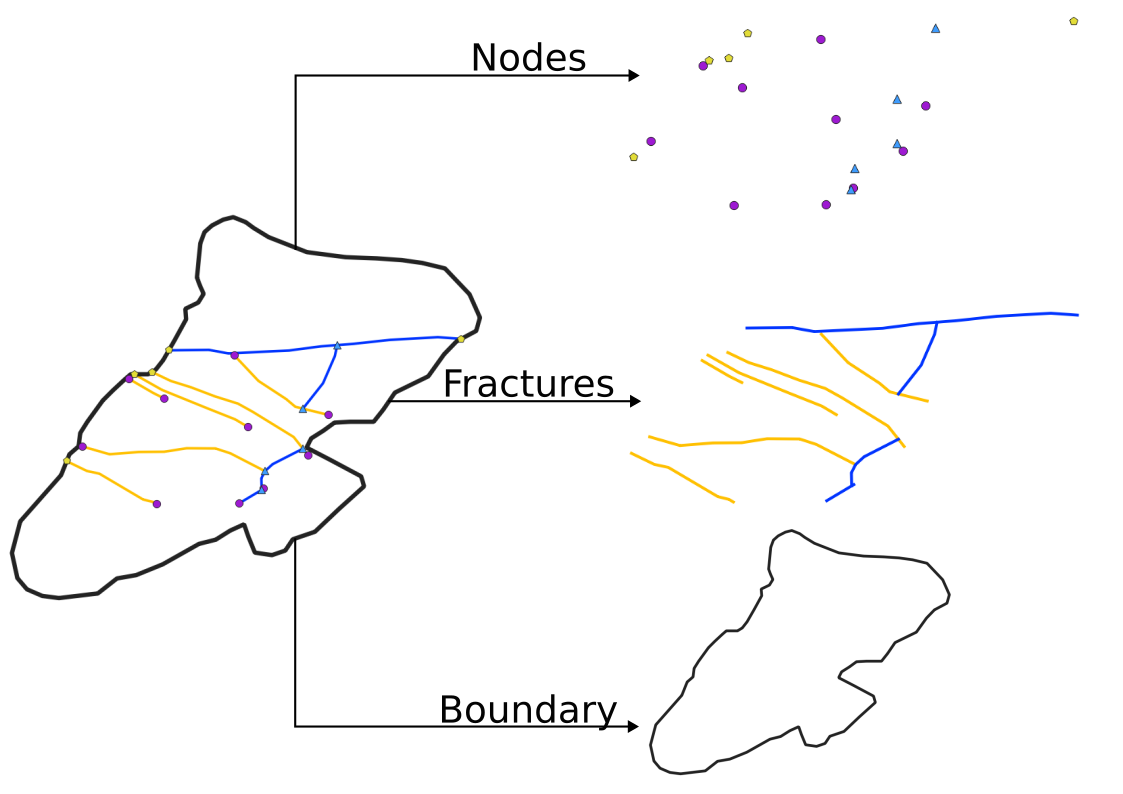
\includegraphics[width=\textwidth]{images/frac_net.png}
		\caption{Structure of a fracture network}\label{fig: fn_struct}
	\end{figure}
	
	\subsection{DFNs}
	
	\section{Statistical background}
	
	\subsection{Survival analysis}
	\subsection{Censoring}
	
	
	\section{Methods}
	
	\subsection{Dimension shift}
	\subsection{Effects on the distribution estimation}
	\subsection{Testing techniques}
				
	
	\newpage
	\printbibliography
	

\end{document}